\section{Anhang}
\label{sec:anhang}

\begin{figure}[H]
\centering
	\begin{subfigure}[t]{0.4\textwidth}
	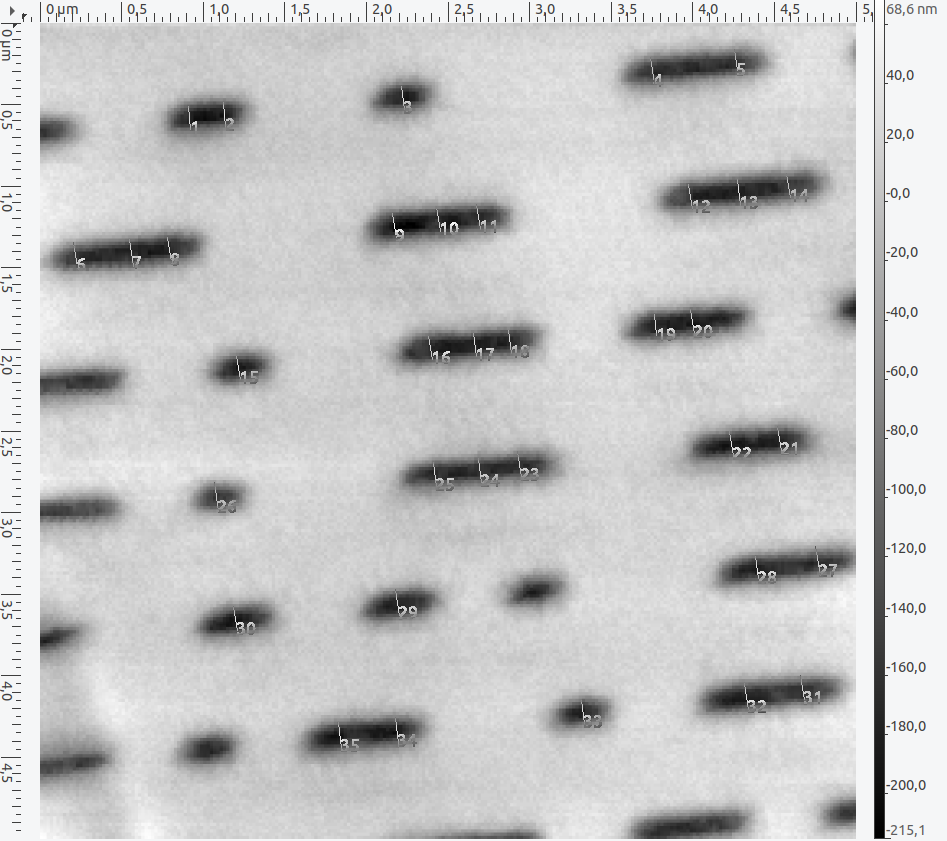
\includegraphics[width=\textwidth]{AFM_auswertung/dvd_breite.png}
	\caption{Bestimmung der durchschnittlichen Pitbreite einer DVD.}
	\end{subfigure}
	~
	\begin{subfigure}[t]{0.4\textwidth}
	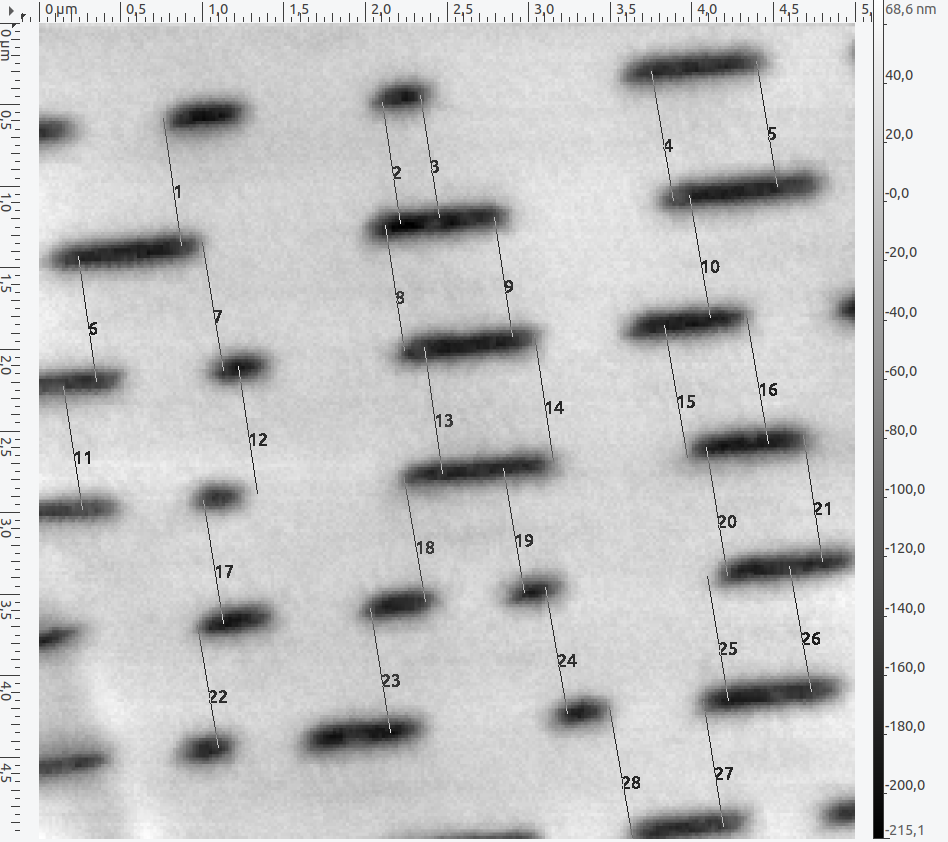
\includegraphics[width=\textwidth]{AFM_auswertung/dvd_abstand.png}
	\caption{Bestimmung des Spurabstands zwischen zwei Pitspuren.}
	\end{subfigure}
	\\
	\begin{subfigure}[t]{0.4\textwidth}
	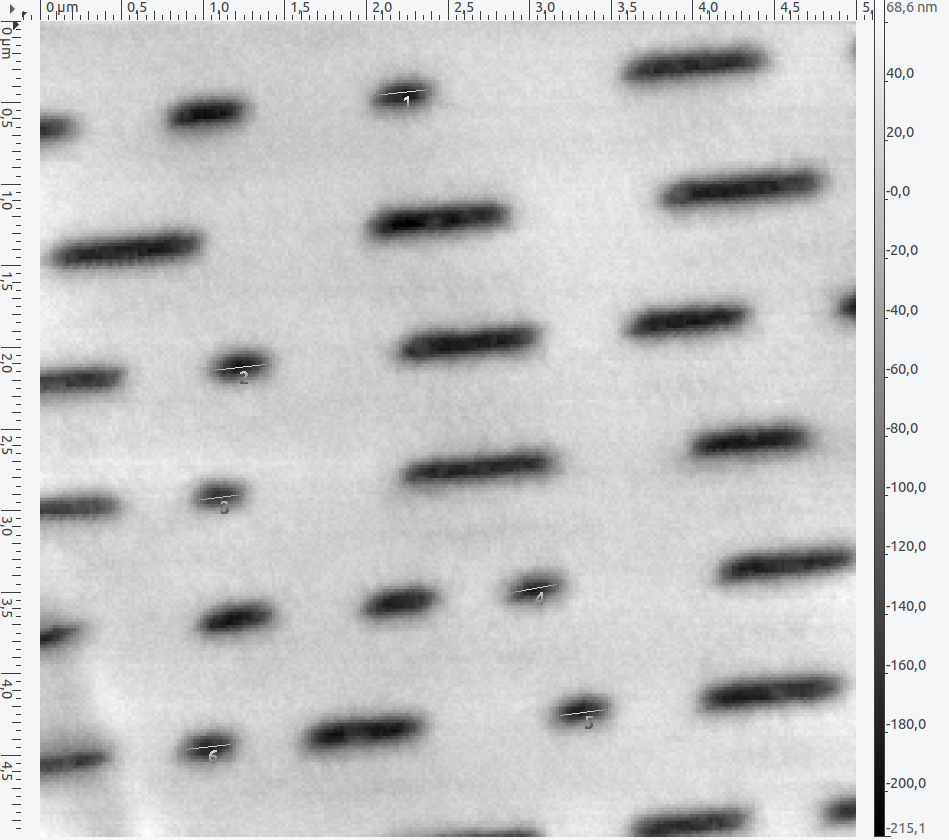
\includegraphics[width=\textwidth]{AFM_auswertung/dvd_Lmin.png}
	\caption{Vermessung der minimalen L\"ange eines Pits auf einer DVD.}
	\end{subfigure}
	~
	\begin{subfigure}[t]{0.4\textwidth}
	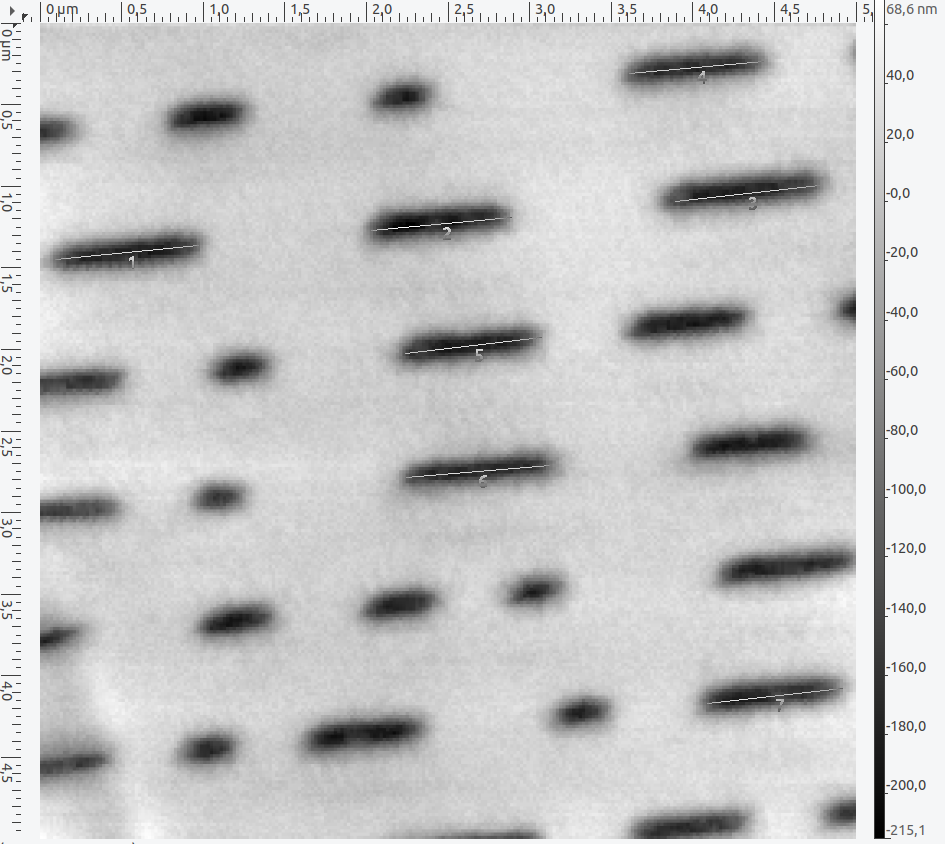
\includegraphics[width=\textwidth]{AFM_auswertung/dvd_Lmax.png}
	\caption{Vermessung der maximalen Pitl\"ange.}
	\end{subfigure}
\caption{Gezeigt ist hier die Vermessung der Pits einer DVD.}
\label{abb:DVD}
\end{figure}


\begin{figure}[H]
\centering
	\begin{subfigure}[t]{0.4\textwidth}
	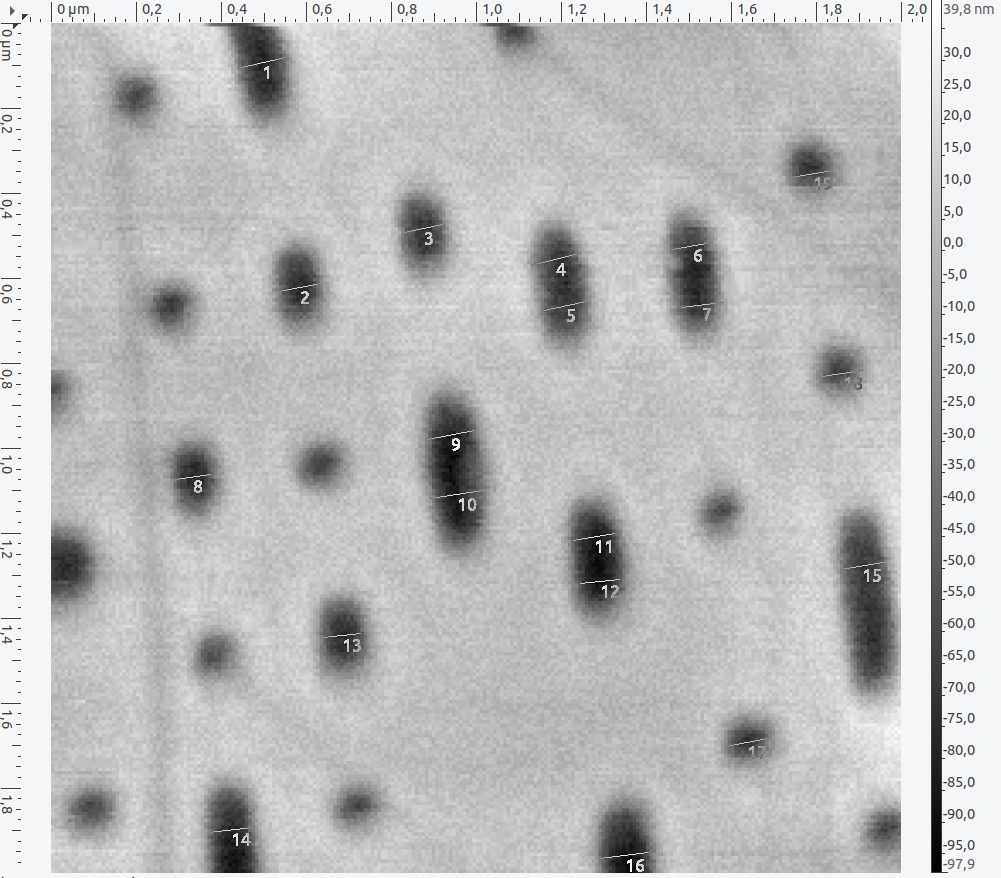
\includegraphics[width=\textwidth]{AFM_auswertung/bluray_breite.png}
	\caption{Bestimmung der durchschnittlichen Pitbreite einer Blu-ray.}
	\end{subfigure}
	~
	\begin{subfigure}[t]{0.4\textwidth}
	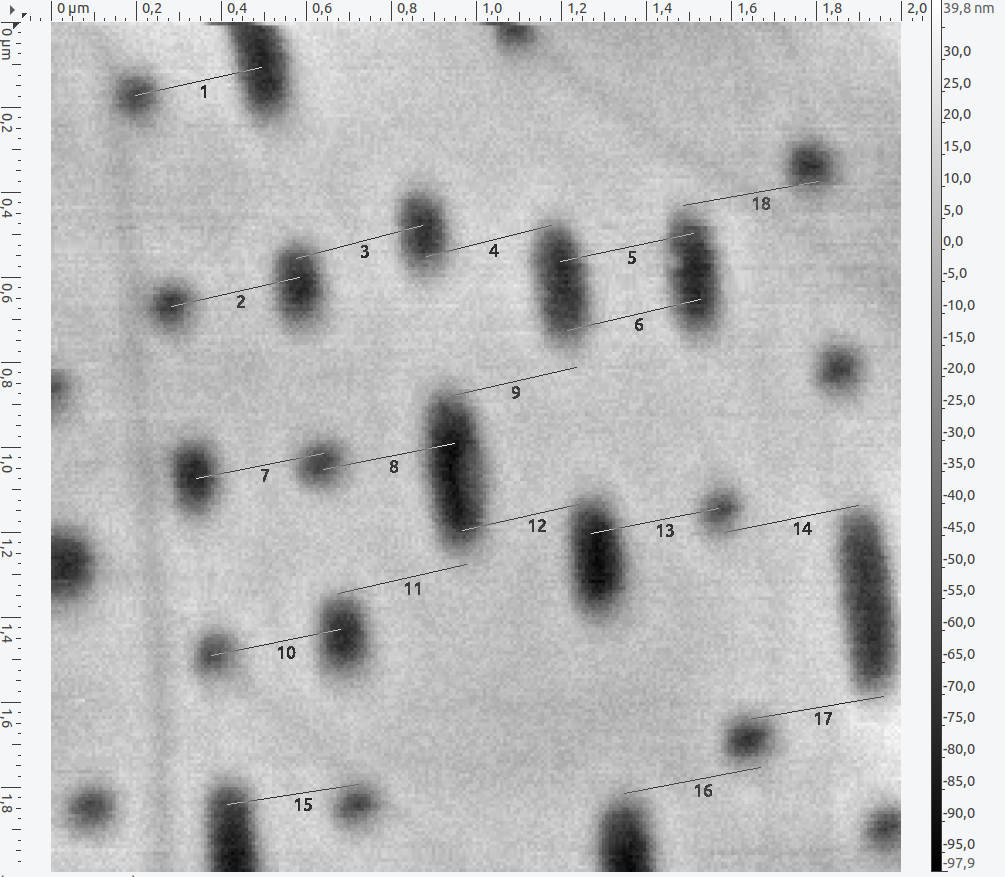
\includegraphics[width=\textwidth]{AFM_auswertung/bluray_abstand.png}
	\caption{Bestimmung des Spurabstands zwischen zwei Pitspuren.}
	\end{subfigure}
	\\
	\begin{subfigure}[t]{0.4\textwidth}
	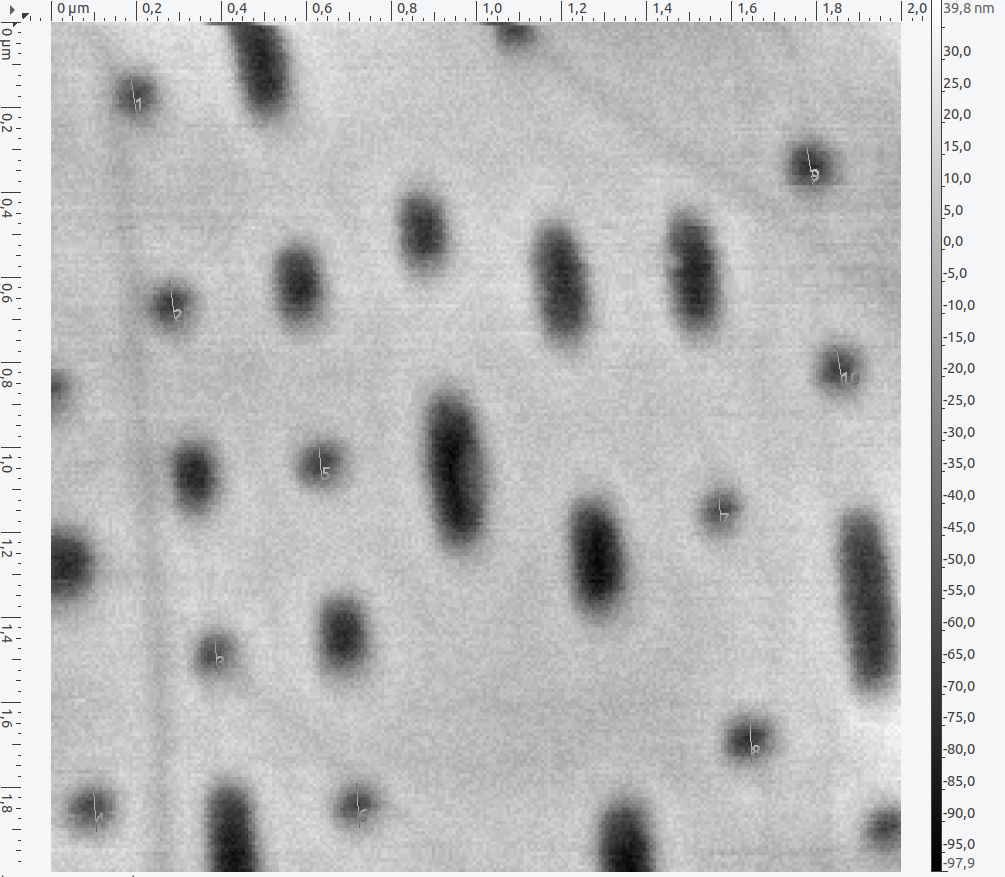
\includegraphics[width=\textwidth]{AFM_auswertung/bluray_Lmin.png}
	\caption{Vermessung der minimalen L\"ange eines Pits auf einer Blu-ray.}
	\end{subfigure}
	~
	\begin{subfigure}[t]{0.4\textwidth}
	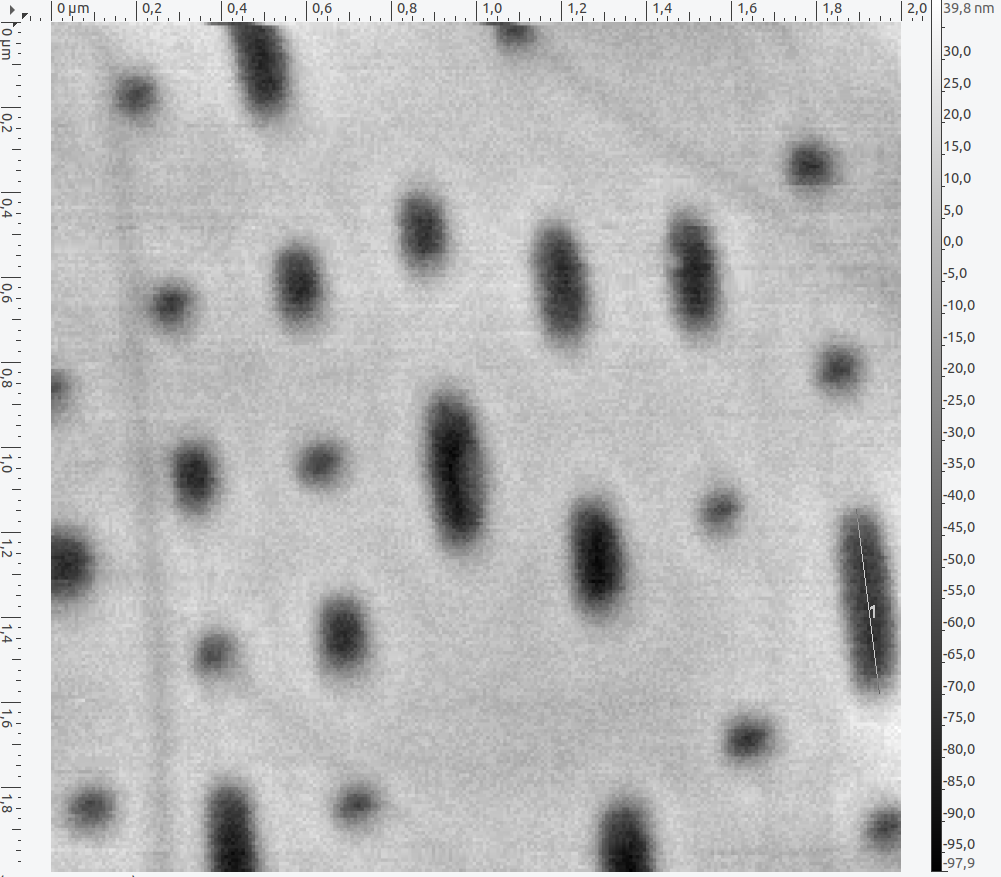
\includegraphics[width=\textwidth]{AFM_auswertung/bluray_Lmax.png}
	\caption{Vermessung der maximalen Pitl\"ange.}
	\end{subfigure}
\caption{Gezeigt ist hier die Vermessung der Pits einer Blu-ray.}
\label{abb:BluRay}
\end{figure}
